%%%%%%%%%%%%%%%%%%%%%%%%%%%%%%%%%%%%%%%%%%%%%%%%%%%%%%%
%% GUIA LOCAL INTELIGENTE - ANÁLISE END TO END
%% UNINASSAU - CIÊNCIA DA COMPUTAÇÃO
%% MODELO ABNTEX2 - OVERLEAF
%%%%%%%%%%%%%%%%%%%%%%%%%%%%%%%%%%%%%%%%%%%%%%%%%%%%%%%

\documentclass[
    12pt,
    oneside,
    openright,
    a4paper,
    english,
    brazil
]{abntex2}

%%%%%%%%%%%%%%%%%%%%%%%%%%%%%%%%%%%%%%%%%%%%%%%%%%%%%
%%                  PACOTES                        %%
%%%%%%%%%%%%%%%%%%%%%%%%%%%%%%%%%%%%%%%%%%%%%%%%%%%%%

\usepackage[utf8]{inputenc}
\usepackage[T1]{fontenc}
\usepackage{graphicx}
\usepackage{float}
\usepackage{amsmath}
\usepackage{array}
\usepackage{booktabs}
\usepackage{longtable}
\usepackage{xcolor}
\usepackage{listings}
\usepackage{setspace}
\usepackage{hyperref}
\usepackage{indentfirst}
\usepackage{caption}
\usepackage{etoolbox}
\usepackage{enumitem}
\usepackage{multirow}
\usepackage{pdflscape}
\usepackage{tikz}
\usetikzlibrary{arrows.meta, positioning, shapes.geometric, fit}

\graphicspath{{Imagens/}}

%%%%%%%%%%%%%%%%%%%%%%%%%%%%%%%%%%%%%%%%%%%%%%%%%%%%%
%%            CONFIGURAÇÕES GERAIS                %%
%%%%%%%%%%%%%%%%%%%%%%%%%%%%%%%%%%%%%%%%%%%%%%%%%%%%%

\OnehalfSpacing

\hypersetup{
    colorlinks=true,
    linkcolor=blue,
    urlcolor=blue,
    citecolor=blue,
    pdftitle={Análise End-to-End do Guia Local Inteligente},
    pdfauthor={Ruan Carlos},
    pdfsubject={Arquitetura, Frontend, Backend, API REST e integrações externas},
    pdfkeywords={React, Vite, Express, Prisma, BetterAuth, PostgreSQL, APIs externas}
}

%%%%%%%%%%%%%%%%%%%%%%%%%%%%%%%%%%%%%%%%%%%%%%%%%%%%%
%%        REMOVE PÁGINAS EM BRANCO                %%
%%%%%%%%%%%%%%%%%%%%%%%%%%%%%%%%%%%%%%%%%%%%%%%%%%%%%

\makeatletter
\patchcmd{\chapter}
{\if@openright\cleardoublepage\else\clearpage\fi}
{\clearpage}{}{}
\makeatother

%%%%%%%%%%%%%%%%%%%%%%%%%%%%%%%%%%%%%%%%%%%%%%%%%%%%%
%%         CONFIGURAÇÃO DE CÓDIGOS                %%
%%%%%%%%%%%%%%%%%%%%%%%%%%%%%%%%%%%%%%%%%%%%%%%%%%%%%

\definecolor{codegreen}{rgb}{0,0.45,0}
\definecolor{codeblue}{rgb}{0.05,0.15,0.7}
\definecolor{codegray}{rgb}{0.45,0.45,0.45}
\definecolor{backgray}{rgb}{0.97,0.97,0.97}

\lstdefinestyle{mystyle}{
    backgroundcolor=\color{backgray},
    commentstyle=\color{codegreen},
    keywordstyle=\color{codeblue}\bfseries,
    numberstyle=\tiny\color{codegray},
    stringstyle=\color{black},
    basicstyle=\ttfamily\footnotesize,
    breaklines=true,
    captionpos=b,
    keepspaces=true,
    numbers=left,
    numbersep=5pt,
    showspaces=false,
    showstringspaces=false,
    showtabs=false,
    tabsize=2,
    frame=single,
    rulecolor=\color{codegray}
}

\lstset{style=mystyle}

%%%%%%%%%%%%%%%%%%%%%%%%%%%%%%%%%%%%%%%%%%%%%%%%%%%%%
%%                  INÍCIO                         %%
%%%%%%%%%%%%%%%%%%%%%%%%%%%%%%%%%%%%%%%%%%%%%%%%%%%%%

\begin{document}

%%%%%%%%%%%%%%%%%%%%%%%%%%%%%%%%%%%%%%%%%%%%%%%%%%%%%
%%                    CAPA                         %%
%%%%%%%%%%%%%%%%%%%%%%%%%%%%%%%%%%%%%%%%%%%%%%%%%%%%%

\begin{capa}
\begin{center}


\includegraphics[width=5cm]{logo-uninassau.png}

\vspace{1cm}

{\large \textbf{CENTRO UNIVERSITÁRIO MAURÍCIO DE NASSAU}}

\vspace{0.3cm}

{\large CURSO DE CIÊNCIA DA COMPUTAÇÃO}

\vspace{3cm}

{\Huge \textbf{GUIA LOCAL INTELIGENTE}}

\vspace{1cm}

{\Large Análise End-to-End da Arquitetura, Frontend, Backend, Banco de Dados e Integrações Externas}

\vspace{3cm}

\textbf{Integrantes}

Ruan Carlos\\
Kauã Nyllo\\
Lucas Silva\\
Bernardo Franco\\

\vfill

Disciplina: Códigos de Alta Performance Web\\
Professor(a): Anderlan Henrique

\vspace{2cm}

Maceió - AL\\
2026

\end{center}
\end{capa}

%%%%%%%%%%%%%%%%%%%%%%%%%%%%%%%%%%%%%%%%%%%%%%%%%%%%%
%%                 CONTRACAPA                      %%
%%%%%%%%%%%%%%%%%%%%%%%%%%%%%%%%%%%%%%%%%%%%%%%%%%%%%

\begin{capa}
\begin{center}

\vspace{4cm}

{\Large \textbf{GUIA LOCAL INTELIGENTE}}

\vspace{4cm}

\begin{flushright}
\begin{minipage}{0.52\textwidth}
Trabalho apresentado ao curso de Ciência da Computação do Centro Universitário Maurício de Nassau — UNINASSAU, como requisito parcial para avaliação acadêmica, contendo análise técnica end-to-end da aplicação Guia Local Inteligente, composta por frontend web, backend REST, autenticação, banco de dados e integração com APIs externas.

\vspace{1cm}

Professor(a): Anderlan Henrique
\end{minipage}
\end{flushright}

\vfill

Maceió - AL\\
2026

\end{center}
\end{capa}

%%%%%%%%%%%%%%%%%%%%%%%%%%%%%%%%%%%%%%%%%%%%%%%%%%%%%
%%                    RESUMO                       %%
%%%%%%%%%%%%%%%%%%%%%%%%%%%%%%%%%%%%%%%%%%%%%%%%%%%%%

\chapter*{Resumo}

Este trabalho apresenta uma análise end-to-end da aplicação \textbf{Guia Local Inteligente}, projeto acadêmico desenvolvido para auxiliar usuários na consulta de informações regionais a partir de um CEP. A solução é dividida em dois repositórios principais: um backend em Node.js, Express, TypeScript, Prisma, PostgreSQL e BetterAuth; e um frontend web em React, TypeScript, Vite, Tailwind CSS e React Router. O sistema permite autenticação social com Google, busca de endereço por CEP, consulta de coordenadas geográficas, obtenção de dados climáticos, listagem de estabelecimentos próximos e gerenciamento de favoritos por usuário autenticado. A análise contempla arquitetura geral, fluxo de dados, camadas do sistema, requisitos funcionais e não funcionais, banco de dados, autenticação, integrações externas, telas, componentes, segurança, implantação e pontos de melhoria.

\vspace{0.5cm}

\textbf{Palavras-chave:} Guia Local Inteligente. React. Vite. Express. Prisma. PostgreSQL. BetterAuth. API REST. APIs externas.

%%%%%%%%%%%%%%%%%%%%%%%%%%%%%%%%%%%%%%%%%%%%%%%%%%%%%
%%                   ABSTRACT                      %%
%%%%%%%%%%%%%%%%%%%%%%%%%%%%%%%%%%%%%%%%%%%%%%%%%%%%%

\chapter*{Abstract}

This paper presents an end-to-end analysis of the \textbf{Guia Local Inteligente} application, an academic project designed to help users retrieve regional information based on a Brazilian ZIP code. The solution is divided into two main repositories: a backend built with Node.js, Express, TypeScript, Prisma, PostgreSQL and BetterAuth; and a web frontend built with React, TypeScript, Vite, Tailwind CSS and React Router. The system supports Google social authentication, address lookup by ZIP code, geocoding, weather data retrieval, nearby place discovery and authenticated favorite place management. This document covers the general architecture, data flow, system layers, functional and non-functional requirements, database, authentication, external integrations, user interface, security, deployment and improvement opportunities.

\vspace{0.5cm}

\textbf{Keywords:} Local Guide. React. Vite. Express. Prisma. PostgreSQL. BetterAuth. REST API. External APIs.

%%%%%%%%%%%%%%%%%%%%%%%%%%%%%%%%%%%%%%%%%%%%%%%%%%%%%
%%                   SUMÁRIO                       %%
%%%%%%%%%%%%%%%%%%%%%%%%%%%%%%%%%%%%%%%%%%%%%%%%%%%%%

\pdfbookmark[0]{\contentsname}{toc}
\tableofcontents*
\clearpage

%%%%%%%%%%%%%%%%%%%%%%%%%%%%%%%%%%%%%%%%%%%%%%%%%%%%%
%%                 INTRODUÇÃO                      %%
%%%%%%%%%%%%%%%%%%%%%%%%%%%%%%%%%%%%%%%%%%%%%%%%%%%%%

\chapter{Introdução}

\section{Contextualização}

A aplicação \textbf{Guia Local Inteligente} surge em um cenário no qual usuários precisam acessar informações rápidas sobre uma região, como endereço, clima e locais próximos. Em vez de exigir que o usuário pesquise manualmente em diferentes plataformas, a aplicação centraliza essas consultas em uma interface única. A entrada principal do sistema é o CEP informado pelo usuário. A partir dele, o backend busca o endereço, obtém coordenadas geográficas, consulta dados meteorológicos e pesquisa estabelecimentos próximos.

O projeto é dividido em dois repositórios:

\begin{itemize}
    \item \textbf{Guia\_Local\_Inteligente-ApiREST}: backend responsável por autenticação, regras de negócio, integração com banco de dados e comunicação com APIs externas.
    \item \textbf{Guia\_Local\_Inteligente-Client}: frontend web responsável pela experiência visual, navegação, telas, chamadas HTTP e interação do usuário com o sistema.
\end{itemize}

\section{Problema}

Usuários frequentemente precisam consultar várias informações sobre uma região: endereço, cidade, clima atual, temperatura mínima e máxima, locais próximos e pontos de interesse. Normalmente, essas informações ficam espalhadas em serviços diferentes. O problema tratado pelo projeto é: \textbf{como centralizar informações úteis de uma região a partir de um CEP, com autenticação, favoritos e interface simples?}

\section{Justificativa}

O projeto se justifica por unir conceitos importantes de desenvolvimento moderno: arquitetura cliente-servidor, API REST, banco relacional, autenticação social, consumo de APIs públicas, tratamento de erros, responsividade e separação de responsabilidades. Além de ser funcional, o projeto demonstra práticas comuns no mercado, como frontend desacoplado do backend, deploy separado, uso de variáveis de ambiente e persistência em PostgreSQL.

%%%%%%%%%%%%%%%%%%%%%%%%%%%%%%%%%%%%%%%%%%%%%%%%%%%%%
%%                  OBJETIVOS                      %%
%%%%%%%%%%%%%%%%%%%%%%%%%%%%%%%%%%%%%%%%%%%%%%%%%%%%%

\chapter{Objetivos}

\section{Objetivo Geral}

Analisar detalhadamente a aplicação Guia Local Inteligente de ponta a ponta, descrevendo sua arquitetura, tecnologias, fluxos, camadas, banco de dados, autenticação, integrações externas, frontend, backend e oportunidades de evolução.

\section{Objetivos Específicos}

\begin{itemize}
    \item Identificar as tecnologias utilizadas no frontend e no backend;
    \item Descrever a arquitetura cliente-servidor da aplicação;
    \item Explicar o fluxo completo de autenticação com Google via BetterAuth;
    \item Detalhar o fluxo de busca por CEP e integração com APIs externas;
    \item Analisar o funcionamento do sistema de favoritos;
    \item Mapear as entidades do banco de dados;
    \item Documentar requisitos funcionais e não funcionais;
    \item Apontar pontos fortes, limitações e melhorias futuras.
\end{itemize}

%%%%%%%%%%%%%%%%%%%%%%%%%%%%%%%%%%%%%%%%%%%%%%%%%%%%%
%%             VISÃO GERAL DO SISTEMA              %%
%%%%%%%%%%%%%%%%%%%%%%%%%%%%%%%%%%%%%%%%%%%%%%%%%%%%%

\chapter{Visão Geral do Sistema}

\section{Descrição do Produto}

O Guia Local Inteligente é uma aplicação web que permite que um usuário autenticado pesquise uma região por CEP. O sistema retorna informações de endereço, clima e locais próximos. A aplicação também permite salvar estabelecimentos favoritos, vinculando esses locais ao usuário logado.

\section{Repositórios Analisados}

\begin{longtable}{|p{4cm}|p{10cm}|}
\hline
\textbf{Repositório} & \textbf{Responsabilidade} \\
\hline
\texttt{Guia\_Local\_Inteligente-ApiREST} & Backend da aplicação. Contém servidor Express, configuração do BetterAuth, Prisma, modelos do banco, rotas de busca e rotas de favoritos. \\
\hline
\texttt{Guia\_Local\_Inteligente-Client} & Frontend web. Contém aplicação React com Vite, telas, componentes visuais, providers, hooks, configuração de autenticação e comunicação HTTP com o backend. \\
\hline
\end{longtable}

\section{Principais Funcionalidades}

\begin{itemize}
    \item Login social com Google;
    \item Controle de sessão por cookies;
    \item Busca de região por CEP;
    \item Consulta de endereço por ViaCEP;
    \item Consulta de coordenadas por Open-Meteo Geocoding;
    \item Consulta de clima por Open-Meteo Forecast;
    \item Consulta de locais próximos por Overpass API/OpenStreetMap;
    \item Exibição de resultados na interface;
    \item Modal/detalhamento de local;
    \item Cadastro, listagem e remoção de favoritos;
    \item Navegação entre início, favoritos, sobre e login.
\end{itemize}

%%%%%%%%%%%%%%%%%%%%%%%%%%%%%%%%%%%%%%%%%%%%%%%%%%%%%
%%                 ARQUITETURA                     %%
%%%%%%%%%%%%%%%%%%%%%%%%%%%%%%%%%%%%%%%%%%%%%%%%%%%%%

\chapter{Arquitetura da Aplicação}

\section{Estilo Arquitetural}

A aplicação adota uma arquitetura \textbf{cliente-servidor}, com separação entre frontend e backend. O frontend é responsável pela interface e pela experiência do usuário. O backend concentra regras de negócio, autenticação, acesso ao banco de dados e chamadas para serviços externos. Essa divisão facilita manutenção, escalabilidade e organização do projeto.

\section{Arquitetura em Camadas}

A solução pode ser compreendida em cinco camadas principais:

\begin{enumerate}
    \item \textbf{Camada de Apresentação}: React, componentes, páginas e estilização.
    \item \textbf{Camada de Estado e Hooks}: providers, hooks de busca, favoritos e autenticação.
    \item \textbf{Camada de API Backend}: Express, rotas REST e middlewares.
    \item \textbf{Camada de Serviços}: regras de negócio, orquestração de APIs externas e operações com favoritos.
    \item \textbf{Camada de Persistência}: Prisma ORM e PostgreSQL.
\end{enumerate}

\section{Diagrama Geral da Arquitetura}

\begin{figure}[H]
\centering
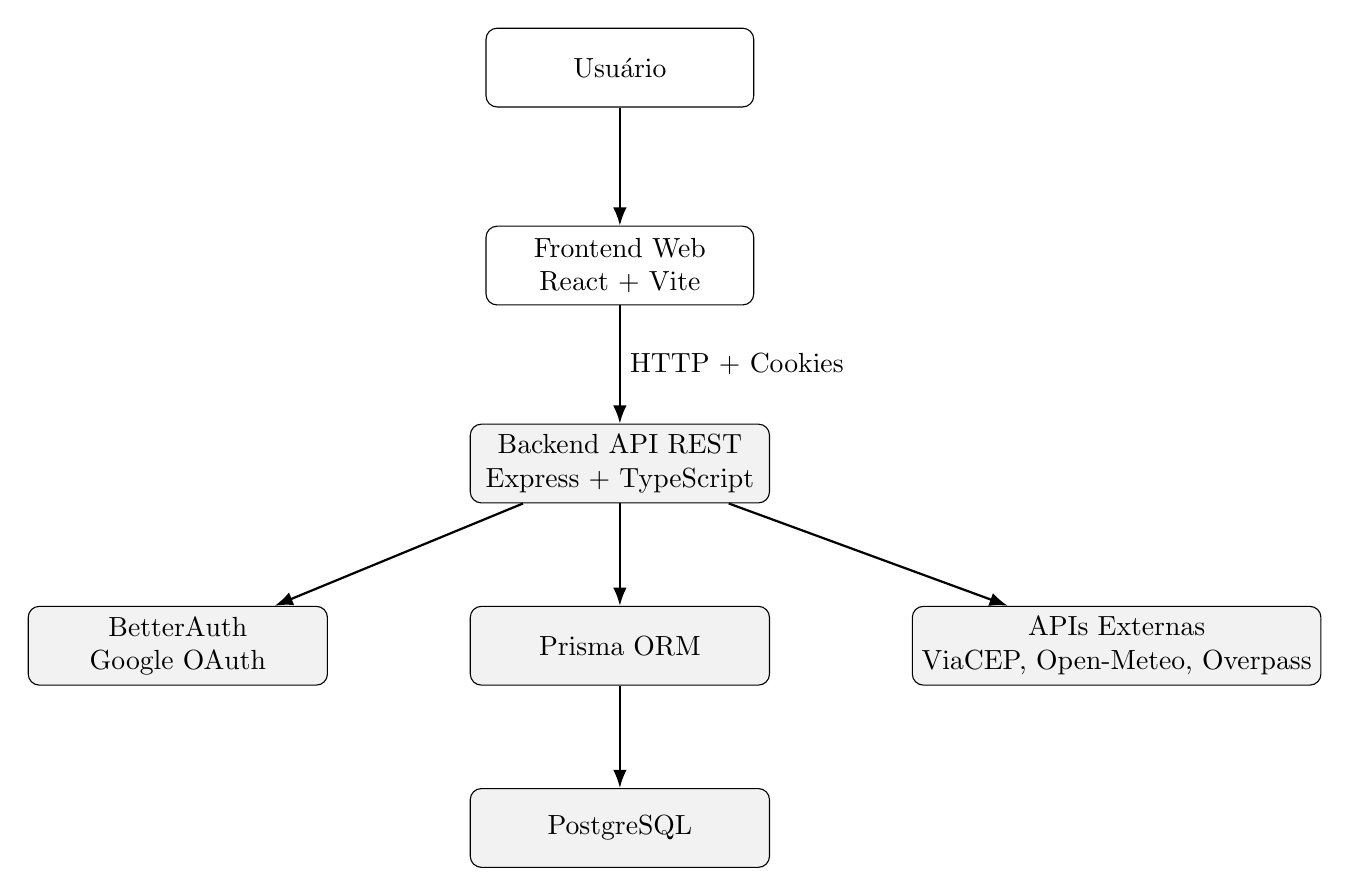
\begin{tikzpicture}[
    node distance=1.5cm,
    box/.style={rectangle, draw, rounded corners, align=center, minimum width=3.4cm, minimum height=1cm},
    api/.style={rectangle, draw, rounded corners, align=center, minimum width=3.8cm, minimum height=1cm, fill=gray!10},
    arrow/.style={-{Latex}, thick}
]

\node[box] (user) {Usuário};
\node[box, below=of user] (front) {Frontend Web\\React + Vite};
\node[api, below=of front] (backend) {Backend API REST\\Express + TypeScript};
\node[api, below left=1.3cm and 1.8cm of backend] (auth) {BetterAuth\\Google OAuth};
\node[api, below=1.3cm of backend] (prisma) {Prisma ORM};
\node[api, below=1.3cm of prisma] (db) {PostgreSQL};
\node[api, below right=1.3cm and 1.8cm of backend] (external) {APIs Externas\\ViaCEP, Open-Meteo, Overpass};

\draw[arrow] (user) -- (front);
\draw[arrow] (front) -- node[right]{HTTP + Cookies} (backend);
\draw[arrow] (backend) -- (auth);
\draw[arrow] (backend) -- (prisma);
\draw[arrow] (prisma) -- (db);
\draw[arrow] (backend) -- (external);

\end{tikzpicture}
\caption{Arquitetura geral do Guia Local Inteligente}
\end{figure}

%%%%%%%%%%%%%%%%%%%%%%%%%%%%%%%%%%%%%%%%%%%%%%%%%%%%%
%%              TECNOLOGIAS UTILIZADAS             %%
%%%%%%%%%%%%%%%%%%%%%%%%%%%%%%%%%%%%%%%%%%%%%%%%%%%%%

\chapter{Tecnologias Utilizadas}

\section{Frontend}

O frontend utiliza tecnologias modernas do ecossistema JavaScript/TypeScript:

\begin{longtable}{|p{4cm}|p{10cm}|}
\hline
\textbf{Tecnologia} & \textbf{Função no Projeto} \\
\hline
React & Construção da interface baseada em componentes reutilizáveis. \\
\hline
TypeScript & Tipagem estática para reduzir erros e melhorar manutenção. \\
\hline
Vite & Ferramenta de build e desenvolvimento rápido. \\
\hline
React Router DOM & Controle de navegação entre páginas como início, login, favoritos e sobre. \\
\hline
Tailwind CSS & Estilização utilitária e responsiva. \\
\hline
Axios & Cliente HTTP configurado para comunicação com a API. \\
\hline
BetterAuth React Client & Cliente de autenticação usado no frontend para sessão, login social e logout. \\
\hline
Lucide React & Ícones utilizados na interface. \\
\hline
Vaul / Base UI / Shadcn & Apoio na construção de componentes interativos, modais e elementos de interface. \\
\hline
\end{longtable}

\section{Backend}

O backend foi desenvolvido com foco em API REST, autenticação e persistência:

\begin{longtable}{|p{4cm}|p{10cm}|}
\hline
\textbf{Tecnologia} & \textbf{Função no Projeto} \\
\hline
Node.js & Ambiente de execução JavaScript no servidor. \\
\hline
Express & Framework HTTP responsável por rotas, middlewares e respostas da API. \\
\hline
TypeScript & Tipagem e organização do código backend. \\
\hline
BetterAuth & Autenticação com Google, sessão e gerenciamento de usuários. \\
\hline
Prisma ORM & Mapeamento objeto-relacional e acesso ao banco PostgreSQL. \\
\hline
PostgreSQL & Banco de dados relacional para usuários, sessões, contas e favoritos. \\
\hline
CORS & Controle de origem permitida e envio de credenciais entre frontend e backend. \\
\hline
Dotenv & Leitura de variáveis de ambiente. \\
\hline
\end{longtable}

%%%%%%%%%%%%%%%%%%%%%%%%%%%%%%%%%%%%%%%%%%%%%%%%%%%%%
%%            ESTRUTURA DOS PROJETOS               %%
%%%%%%%%%%%%%%%%%%%%%%%%%%%%%%%%%%%%%%%%%%%%%%%%%%%%%

\chapter{Estrutura dos Projetos}

\section{Estrutura do Backend}

A organização do backend segue separação por responsabilidades:

\begin{lstlisting}[language=bash, caption={Estrutura resumida do backend}]
Guia_Local_Inteligente-ApiREST/
├── prisma/
│   └── schema.prisma
├── src/
│   ├── @types/
│   ├── controllers/
│   │   ├── favorite.controller.ts
│   │   └── search.controller.ts
│   ├── lib/
│   │   ├── auth.ts
│   │   ├── get-session-user.ts
│   │   └── prisma.ts
│   ├── routes/
│   │   ├── favorite.route.ts
│   │   └── search.route.ts
│   ├── services/
│   │   ├── favorite.service.ts
│   │   └── search.service.ts
│   ├── app.ts
│   └── server.ts
├── package.json
├── prisma.config.ts
└── tsconfig.json
\end{lstlisting}

\section{Estrutura do Frontend}

O frontend é organizado em componentes, páginas, hooks, providers, interfaces e bibliotecas auxiliares:

\begin{lstlisting}[language=bash, caption={Estrutura resumida do frontend}]
Guia_Local_Inteligente-Client/
├── public/
├── src/
│   ├── assets/
│   ├── components/
│   │   ├── pages/
│   │   │   ├── inicio/
│   │   │   ├── favoritos/
│   │   │   ├── login/
│   │   │   └── sobre/
│   │   ├── modals/
│   │   └── navigationMobile/
│   ├── hooks/
│   │   ├── useSearch.ts
│   │   └── useFavorites.ts
│   ├── interfaces/
│   ├── lib/
│   │   ├── axios.ts
│   │   └── auth-client.ts
│   ├── providers/
│   │   ├── AuthProvider.tsx
│   │   └── FavoritesProvider.tsx
│   ├── utils/
│   ├── App.tsx
│   ├── index.css
│   └── main.tsx
├── Dockerfile
├── docker-compose.yml
├── nginx.conf
├── package.json
└── vite.config.ts
\end{lstlisting}

%%%%%%%%%%%%%%%%%%%%%%%%%%%%%%%%%%%%%%%%%%%%%%%%%%%%%
%%          LEVANTAMENTO DE REQUISITOS             %%
%%%%%%%%%%%%%%%%%%%%%%%%%%%%%%%%%%%%%%%%%%%%%%%%%%%%%

\chapter{Levantamento de Requisitos}

\section{Requisitos Funcionais}

\begin{longtable}{|p{2cm}|p{12cm}|}
\hline
\textbf{Código} & \textbf{Descrição} \\
\hline
RF01 & O sistema deve permitir login social com conta Google. \\
\hline
RF02 & O sistema deve manter sessão do usuário por meio do BetterAuth e cookies. \\
\hline
RF03 & O sistema deve permitir consulta de região por CEP. \\
\hline
RF04 & O sistema deve validar se o CEP possui 8 dígitos numéricos. \\
\hline
RF05 & O sistema deve consultar endereço a partir da API ViaCEP. \\
\hline
RF06 & O sistema deve obter coordenadas da cidade por meio da API de geocodificação da Open-Meteo. \\
\hline
RF07 & O sistema deve consultar clima atual, temperatura mínima e máxima. \\
\hline
RF08 & O sistema deve buscar locais próximos usando a Overpass API/OpenStreetMap. \\
\hline
RF09 & O sistema deve apresentar os resultados da busca no frontend. \\
\hline
RF10 & O sistema deve permitir salvar locais como favoritos. \\
\hline
RF11 & O sistema deve listar favoritos do usuário autenticado. \\
\hline
RF12 & O sistema deve permitir remover um favorito. \\
\hline
RF13 & O sistema deve impedir acesso às rotas de busca e favoritos por usuários não autenticados. \\
\hline
RF14 & O sistema deve possuir navegação entre início, favoritos, sobre e login. \\
\hline
RF15 & O sistema deve exibir estados de carregamento, sucesso e erro durante a busca. \\
\hline
\end{longtable}

\section{Requisitos Não Funcionais}

\begin{longtable}{|p{2cm}|p{12cm}|}
\hline
\textbf{Código} & \textbf{Descrição} \\
\hline
RNF01 & A aplicação deve ser responsiva, com foco em uso web/mobile. \\
\hline
RNF02 & A comunicação entre frontend e backend deve utilizar HTTP/HTTPS. \\
\hline
RNF03 & A autenticação deve utilizar cookies seguros em produção. \\
\hline
RNF04 & O backend deve validar variáveis de ambiente obrigatórias no momento da inicialização. \\
\hline
RNF05 & O banco de dados deve manter integridade referencial entre usuários, sessões, contas e favoritos. \\
\hline
RNF06 & O sistema deve tratar erros de APIs externas e retornar mensagens compreensíveis. \\
\hline
RNF07 & A aplicação deve manter o frontend desacoplado do backend. \\
\hline
RNF08 & O código deve ser organizado em camadas para facilitar manutenção. \\
\hline
RNF09 & A API deve permitir CORS apenas para a origem configurada no ambiente. \\
\hline
RNF10 & O sistema deve ser preparado para deploy em serviços como Vercel, Render ou infraestrutura similar. \\
\hline
\end{longtable}

%%%%%%%%%%%%%%%%%%%%%%%%%%%%%%%%%%%%%%%%%%%%%%%%%%%%%
%%                 BACKEND                         %%
%%%%%%%%%%%%%%%%%%%%%%%%%%%%%%%%%%%%%%%%%%%%%%%%%%%%%

\chapter{Análise do Backend}

\section{Visão Geral}

O backend é uma API REST construída com Express e TypeScript. Ele expõe rotas para autenticação, verificação de saúde, consulta de usuário atual, busca por CEP e gerenciamento de favoritos. A aplicação utiliza BetterAuth para autenticação, Prisma para comunicação com PostgreSQL e serviços internos para organizar as regras de negócio.

\section{Scripts do Backend}

O arquivo \texttt{package.json} do backend define os comandos principais:

\begin{lstlisting}[language=json, caption={Scripts principais do backend}]
{
  "dev": "tsx watch src/server.ts",
  "build": "npm run prisma:generate && tsc",
  "start": "node dist/server.js",
  "prisma:generate": "prisma generate",
  "prisma:deploy": "prisma migrate deploy",
  "prisma:push": "prisma db push",
  "prisma:studio": "prisma studio"
}
\end{lstlisting}

Esses scripts mostram que o backend possui fluxo de desenvolvimento com \texttt{tsx watch}, build com geração do Prisma Client e compilação TypeScript, além de comandos específicos para migração e inspeção do banco.

\section{Configuração da Aplicação Express}

O arquivo \texttt{src/app.ts} centraliza a configuração do servidor Express. Ele configura CORS, BetterAuth, JSON parser, health check e rotas de domínio:

\begin{lstlisting}[language=JavaScript, caption={Configuração resumida do Express}]
const app = express();

app.use(cors({
  origin: allowedOrigins,
  methods: ["GET", "POST", "PUT", "DELETE"],
  credentials: true,
}));

app.all(/\/api\/auth\/.*/, toNodeHandler(auth));
app.use(express.json());

app.get("/api/health", (req, res) => {
  res.json({ ok: true });
});

app.use("/api/favorites", favoriteRoutes);
app.use("/api/search", searchRoutes);
\end{lstlisting}

A ordem é importante: o handler do BetterAuth é registrado antes do \texttt{express.json()}, pois bibliotecas de autenticação podem exigir leitura específica da requisição. Depois são registradas as rotas de negócio.

\section{CORS e Credenciais}

O backend usa a variável \texttt{FRONTEND\_URL} para montar a lista de origens permitidas. O CORS está configurado com \texttt{credentials: true}, permitindo que cookies de sessão sejam enviados entre frontend e backend. Essa configuração é indispensável para login persistente quando frontend e backend estão em domínios diferentes.

\section{Health Check}

A rota \texttt{/api/health} retorna \texttt{{ ok: true }}. Ela serve para verificar se a API está online, sendo útil em deploys, monitoramento e testes rápidos.

\section{Rota de Usuário Atual}

A rota \texttt{/api/me} consulta a sessão atual através do BetterAuth e retorna os dados da sessão. Ela é útil para validar se o usuário está logado e para obter informações do usuário autenticado.

%%%%%%%%%%%%%%%%%%%%%%%%%%%%%%%%%%%%%%%%%%%%%%%%%%%%%
%%              AUTENTICAÇÃO                       %%
%%%%%%%%%%%%%%%%%%%%%%%%%%%%%%%%%%%%%%%%%%%%%%%%%%%%%

\chapter{Autenticação e Sessão}

\section{BetterAuth no Backend}

A autenticação é configurada em \texttt{src/lib/auth.ts}. O backend exige as seguintes variáveis de ambiente:

\begin{itemize}
    \item \texttt{DATABASE\_URL}
    \item \texttt{BETTER\_AUTH\_SECRET}
    \item \texttt{BETTER\_AUTH\_URL}
    \item \texttt{FRONTEND\_URL}
    \item \texttt{GOOGLE\_CLIENT\_ID}
    \item \texttt{GOOGLE\_CLIENT\_SECRET}
\end{itemize}

Essa validação em tempo de inicialização é positiva, pois evita que a aplicação suba com configuração incompleta. O BetterAuth é configurado com adaptador Prisma, provedor PostgreSQL e login social com Google.

\begin{lstlisting}[language=JavaScript, caption={Configuração resumida do BetterAuth}]
export const auth = betterAuth({
  appName: "GLI",
  baseURL: process.env.BETTER_AUTH_URL,
  trustedOrigins: [process.env.FRONTEND_URL],
  advanced: {
    defaultCookieAttributes: {
      sameSite: "none",
      secure: true,
    },
  },
  database: prismaAdapter(prisma, { provider: "postgresql" }),
  socialProviders: {
    google: {
      clientId: process.env.GOOGLE_CLIENT_ID,
      clientSecret: process.env.GOOGLE_CLIENT_SECRET,
    },
  },
});
\end{lstlisting}

\section{BetterAuth no Frontend}

No frontend, o cliente de autenticação é criado com \texttt{createAuthClient}, apontando para a URL da API:

\begin{lstlisting}[language=JavaScript, caption={Cliente de autenticação no frontend}]
export const authClient = createAuthClient({
  baseURL: import.meta.env.VITE_API_URL || "http://localhost:3000",
});
\end{lstlisting}

O \texttt{AuthProvider} encapsula o estado de autenticação, consulta a sessão com \texttt{authClient.useSession()} e disponibiliza funções de login e logout para a aplicação.

\section{Fluxo de Login com Google}

O fluxo de autenticação ocorre da seguinte forma:

\begin{enumerate}
    \item O usuário acessa a tela de login.
    \item O frontend chama \texttt{signInWithGoogle()}.
    \item O BetterAuth redireciona o usuário para o provedor Google.
    \item Após autorização, o Google retorna para o backend.
    \item O BetterAuth cria ou atualiza usuário, conta e sessão no banco.
    \item O backend grava cookies de sessão.
    \item O usuário retorna ao frontend na URL definida em \texttt{callbackURL}.
    \item O frontend passa a reconhecer o usuário por \texttt{authClient.useSession()}.
\end{enumerate}

\section{Middleware de Proteção de Rotas}

O backend possui um middleware \texttt{requireAuth}. Ele consulta a sessão usando os cabeçalhos da requisição e bloqueia usuários não autenticados:

\begin{lstlisting}[language=JavaScript, caption={Middleware requireAuth}]
export async function requireAuth(req, res, next) {
  const user = await getSessionUser(req);

  if (!user) {
    return res.status(401).json({
      message: "Usuário não autenticado.",
    });
  }

  req.user = user;
  next();
}
\end{lstlisting}

Esse middleware é aplicado nas rotas de busca e favoritos, tornando a autenticação obrigatória para essas funcionalidades.

%%%%%%%%%%%%%%%%%%%%%%%%%%%%%%%%%%%%%%%%%%%%%%%%%%%%%
%%             BANCO DE DADOS                      %%
%%%%%%%%%%%%%%%%%%%%%%%%%%%%%%%%%%%%%%%%%%%%%%%%%%%%%

\chapter{Banco de Dados e Modelo Relacional}

\section{Prisma e PostgreSQL}

O projeto utiliza Prisma como ORM e PostgreSQL como banco relacional. O \texttt{schema.prisma} define modelos relacionados à autenticação e ao domínio de favoritos.

\section{Entidades Principais}

\begin{longtable}{|p{3cm}|p{11cm}|}
\hline
\textbf{Modelo} & \textbf{Descrição} \\
\hline
User & Representa o usuário autenticado. Possui nome, e-mail, imagem, verificação de e-mail e relações com sessões, contas e favoritos. \\
\hline
Session & Representa uma sessão ativa ou expirada, contendo token, data de expiração, IP, user agent e relação com usuário. \\
\hline
Account & Representa a conta vinculada ao provedor de autenticação, como Google. Armazena tokens e metadados da conta. \\
\hline
Verification & Representa registros de verificação usados pela autenticação. \\
\hline
FavoritePlace & Representa um local salvo como favorito por um usuário. Contém nome, categoria, descrição, avaliação, horário e coordenadas. \\
\hline
\end{longtable}

\section{Modelo FavoritePlace}

O modelo \texttt{FavoritePlace} é central para a funcionalidade de favoritos:

\begin{lstlisting}[language=JavaScript, caption={Modelo FavoritePlace no Prisma}]
model FavoritePlace {
  id String @id @default(cuid())

  userId String
  user   User   @relation(fields: [userId], references: [id], onDelete: Cascade)

  placeId     String
  name        String
  category    String
  description String?
  rating      Float?
  hours       String?
  latitude    Float?
  longitude   Float?

  createdAt DateTime @default(now())
  updatedAt DateTime @updatedAt

  @@unique([userId, placeId])
  @@index([userId])
  @@map("favorite_place")
}
\end{lstlisting}

O índice único \texttt{@@unique([userId, placeId])} impede que o mesmo usuário favorite o mesmo local mais de uma vez. Isso é importante para consistência dos dados.

\section{Relacionamentos}

\begin{itemize}
    \item Um \texttt{User} pode ter várias \texttt{Session}.
    \item Um \texttt{User} pode ter várias \texttt{Account}.
    \item Um \texttt{User} pode ter vários \texttt{FavoritePlace}.
    \item Se um usuário for removido, suas sessões, contas e favoritos são removidos em cascata.
\end{itemize}

\section{Diagrama Entidade-Relacionamento Simplificado}

\begin{figure}[H]
\centering
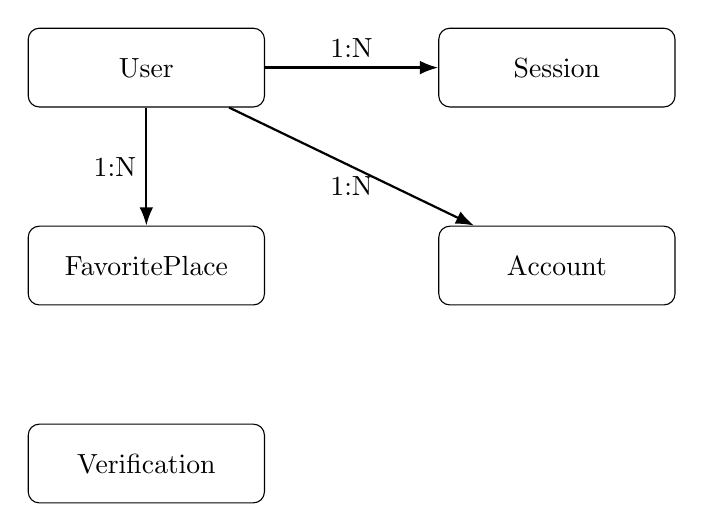
\begin{tikzpicture}[
    entity/.style={rectangle, draw, rounded corners, align=center, minimum width=3cm, minimum height=1cm},
    arrow/.style={-{Latex}, thick}
]
\node[entity] (user) {User};
\node[entity, right=2.2cm of user] (session) {Session};
\node[entity, below=1.5cm of session] (account) {Account};
\node[entity, below=1.5cm of user] (fav) {FavoritePlace};
\node[entity, below=1.5cm of fav] (ver) {Verification};

\draw[arrow] (user) -- node[above]{1:N} (session);
\draw[arrow] (user) -- node[below]{1:N} (account);
\draw[arrow] (user) -- node[left]{1:N} (fav);
\end{tikzpicture}
\caption{Relacionamentos principais do banco de dados}
\end{figure}

%%%%%%%%%%%%%%%%%%%%%%%%%%%%%%%%%%%%%%%%%%%%%%%%%%%%%
%%              BUSCA POR CEP                      %%
%%%%%%%%%%%%%%%%%%%%%%%%%%%%%%%%%%%%%%%%%%%%%%%%%%%%%

\chapter{Fluxo de Busca por CEP}

\section{Visão Geral do Fluxo}

A busca por CEP é a principal funcionalidade do sistema. Ela recebe um CEP, valida a entrada, consulta endereço, transforma a cidade em coordenadas, busca o clima e encontra locais próximos. O backend orquestra tudo em uma única chamada para o frontend.

\section{Fluxo Ponta a Ponta}

\begin{enumerate}
    \item Usuário informa um CEP na tela inicial.
    \item Frontend chama \texttt{GET /api/search/:cep} usando Axios.
    \item Backend verifica se o usuário está autenticado.
    \item Controller valida a existência do CEP na rota.
    \item Service remove caracteres não numéricos e valida 8 dígitos.
    \item Backend chama a API ViaCEP.
    \item Backend obtém cidade e UF do endereço retornado.
    \item Backend chama Open-Meteo Geocoding para obter latitude e longitude.
    \item Backend chama Open-Meteo Forecast para obter clima.
    \item Backend chama Overpass API para obter locais próximos.
    \item Backend monta o objeto final com endereço, clima e locais.
    \item Frontend exibe resultado ou mensagem de erro.
\end{enumerate}

\section{Orquestração no Service}

A função \texttt{searchRegion} é responsável por unir todas as etapas:

\begin{lstlisting}[language=JavaScript, caption={Orquestração da busca no backend}]
export async function searchRegion(cep: string): Promise<SearchResult> {
  const address = await getAddressByCep(cep);
  const coordinates = await getCoordinates(address.localidade);

  const [weather, places] = await Promise.all([
    getWeather(coordinates.latitude, coordinates.longitude),
    getNearbyPlaces(coordinates.latitude, coordinates.longitude).catch(() => []),
  ]);

  return { address, weather, places };
}
\end{lstlisting}

Um ponto positivo é o uso de \texttt{Promise.all} para buscar clima e locais em paralelo. Outro ponto positivo é que, se a busca de locais falhar, o sistema ainda retorna endereço e clima, usando lista vazia para locais.

\section{Validação do CEP}

A validação remove caracteres não numéricos e exige exatamente 8 dígitos:

\begin{lstlisting}[language=JavaScript, caption={Validação do CEP}]
const cleanCep = cep.replace(/\D/g, "");

if (cleanCep.length !== 8 || !/^\d{8}$/.test(cleanCep)) {
  throw new Error("CEP inválido. Informe 8 dígitos numéricos.");
}
\end{lstlisting}

Essa abordagem permite aceitar entradas como \texttt{57000-000}, pois o hífen é removido antes da validação.

\section{Integração com ViaCEP}

A função \texttt{getAddressByCep} consulta:

\begin{center}
\url{https://viacep.com.br/ws/{cep}/json/}
\end{center}

O retorno é convertido para um objeto contendo CEP, logradouro, bairro, localidade e UF. Se o CEP não existir ou os dados vierem incompletos, o service lança erro.

\section{Integração com Open-Meteo Geocoding}

Após obter a cidade no ViaCEP, o backend consulta:

\begin{center}
\url{https://geocoding-api.open-meteo.com/v1/search}
\end{center}

A API retorna latitude e longitude. O backend valida se os valores são numéricos antes de prosseguir.

\section{Integração com Open-Meteo Forecast}

Com latitude e longitude, o backend consulta clima atual e temperaturas diárias:

\begin{lstlisting}[language=JavaScript, caption={Parâmetros de clima}]
const params = new URLSearchParams({
  latitude: String(latitude),
  longitude: String(longitude),
  current: "temperature_2m,weather_code",
  daily: "temperature_2m_max,temperature_2m_min",
  timezone: "auto",
});
\end{lstlisting}

O código meteorológico é traduzido para textos em português, como \texttt{Céu limpo}, \texttt{Nublado}, \texttt{Chuva leve} e \texttt{Pancadas de chuva}.

\section{Integração com Overpass API}

A função \texttt{getNearbyPlaces} monta uma query Overpass para buscar estabelecimentos em um raio padrão de 3000 metros. Entre as categorias pesquisadas estão restaurantes, cafés, lanchonetes, farmácias, hospitais, bancos, mercados, lojas, atrações turísticas, parques, academias, escolas, universidades, postos de combustível e outros.

O resultado é filtrado para locais com nome e convertido para o formato:

\begin{lstlisting}[language=JavaScript, caption={Formato de local retornado ao frontend}]
{
  id: place.id,
  name: place.tags?.name || "Nome não informado",
  category: translateCategory(place),
  description: getDescription(place),
  latitude: place.lat || place.center?.lat || latitude,
  longitude: place.lon || place.center?.lon || longitude,
  rating: null,
  hours: place.tags?.opening_hours || "Horário não informado",
}
\end{lstlisting}

A função retorna no máximo 12 locais, evitando sobrecarregar a interface.

%%%%%%%%%%%%%%%%%%%%%%%%%%%%%%%%%%%%%%%%%%%%%%%%%%%%%
%%              FAVORITOS                          %%
%%%%%%%%%%%%%%%%%%%%%%%%%%%%%%%%%%%%%%%%%%%%%%%%%%%%%

\chapter{Sistema de Favoritos}

\section{Visão Geral}

O sistema de favoritos permite que o usuário autenticado salve locais de interesse. A funcionalidade envolve frontend, backend, middleware de autenticação, controller, service e banco de dados.

\section{Rotas de Favoritos}

As rotas estão protegidas por \texttt{requireAuth}:

\begin{lstlisting}[language=JavaScript, caption={Rotas de favoritos}]
routes.use(requireAuth);
routes.get("/", listFavoritesController);
routes.post("/", createFavoriteController);
routes.delete("/:placeId", deleteFavoriteController);
\end{lstlisting}

\section{Adicionar Favorito}

Para criar um favorito, o backend exige \texttt{placeId}, \texttt{name} e \texttt{category}. Os demais campos são opcionais. O service usa \texttt{upsert}, que atualiza o registro caso ele já exista ou cria um novo caso não exista.

\begin{lstlisting}[language=JavaScript, caption={Upsert de favorito}]
return prisma.favoritePlace.upsert({
  where: {
    userId_placeId: {
      userId: data.userId,
      placeId: data.placeId,
    },
  },
  update: {
    name: data.name,
    category: data.category,
    description: data.description,
    rating: data.rating,
    hours: data.hours,
    latitude: data.latitude,
    longitude: data.longitude,
  },
  create: data,
});
\end{lstlisting}

Essa estratégia é adequada porque evita duplicidade e mantém os dados atualizados.

\section{Listar Favoritos}

A listagem filtra por \texttt{userId} e ordena por data de criação decrescente, mostrando primeiro os favoritos mais recentes.

\section{Remover Favorito}

A remoção usa a chave composta \texttt{userId\_placeId}, garantindo que um usuário só remova seus próprios favoritos.

\section{FavoritesProvider no Frontend}

No frontend, o \texttt{FavoritesProvider} mantém os favoritos em estado global. Ele expõe:

\begin{itemize}
    \item \texttt{favorites}: lista atual de favoritos;
    \item \texttt{isLoading}: estado de carregamento;
    \item \texttt{add}: adiciona favorito;
    \item \texttt{remove}: remove favorito;
    \item \texttt{isFavorite}: verifica se um local já está salvo;
    \item \texttt{refresh}: recarrega a lista.
\end{itemize}

Esse provider evita repetição de lógica nas páginas e componentes.

%%%%%%%%%%%%%%%%%%%%%%%%%%%%%%%%%%%%%%%%%%%%%%%%%%%%%
%%                 FRONTEND                        %%
%%%%%%%%%%%%%%%%%%%%%%%%%%%%%%%%%%%%%%%%%%%%%%%%%%%%%

\chapter{Análise do Frontend}

\section{Visão Geral}

O frontend é uma aplicação React criada com Vite e TypeScript. Ele consome a API backend por Axios, usa BetterAuth para sessão, React Router para navegação e Tailwind CSS para estilização. A proposta visual é moderna, responsiva e centrada em telas principais simples.

\section{Scripts do Frontend}

\begin{lstlisting}[language=json, caption={Scripts principais do frontend}]
{
  "dev": "vite",
  "build": "tsc -b && vite build",
  "lint": "eslint .",
  "preview": "vite preview"
}
\end{lstlisting}

\section{Rotas da Aplicação}

O arquivo \texttt{App.tsx} define as páginas principais:

\begin{lstlisting}[language=JavaScript, caption={Rotas principais do frontend}]
<Routes>
  <Route path="/" element={<InicioPage />} />
  <Route path="/login" element={<LoginPage />} />
  <Route path="/favoritos" element={<FavoritosPage />} />
  <Route path="/sobre" element={<SobrePage />} />
</Routes>
{pathname !== '/login' && <NavigationMobile />}
<PlaceDetailModal />
\end{lstlisting}

A navegação mobile aparece em todas as telas, exceto na tela de login. O modal de detalhes fica global, podendo ser aberto a partir de diferentes partes da interface.

\section{Cliente HTTP}

O arquivo \texttt{src/lib/axios.ts} cria uma instância Axios com \texttt{baseURL} definida por \texttt{VITE\_API\_URL}. O uso de \texttt{withCredentials: true} é essencial para enviar cookies de sessão ao backend.

\begin{lstlisting}[language=JavaScript, caption={Cliente HTTP com credenciais}]
export const api = axios.create({
  baseURL: import.meta.env.VITE_API_URL,
  withCredentials: true,
  headers: {
    "Content-Type": "application/json",
  },
});
\end{lstlisting}

\section{Hook useSearch}

O hook \texttt{useSearch} controla a busca por CEP e os estados de tela:

\begin{itemize}
    \item \texttt{idle}: estado inicial;
    \item \texttt{loading}: busca em andamento;
    \item \texttt{success}: busca concluída com sucesso;
    \item \texttt{error}: falha na busca.
\end{itemize}

Ele chama \texttt{/api/search/:cep}, armazena os dados retornados e trata mensagens de erro vindas do backend.

\section{Providers}

A aplicação utiliza providers para organizar estado global:

\begin{longtable}{|p{4cm}|p{10cm}|}
\hline
\textbf{Provider} & \textbf{Responsabilidade} \\
\hline
AuthProvider & Mantém dados do usuário autenticado, estado de carregamento, login com Google e logout. \\
\hline
FavoritesProvider & Mantém lista de favoritos, adiciona, remove, verifica e recarrega favoritos. \\
\hline
\end{longtable}

\section{Páginas Principais}

\subsection{Tela de Login}

A tela de login é a porta de entrada para autenticação. Ela deve permitir que o usuário inicie login com Google. Após autenticação, o usuário é redirecionado para a página inicial.

\subsection{Tela Inicial}

A tela inicial é onde ocorre a busca por CEP. Ela deve conter campo de entrada, botão de pesquisa, estados visuais de carregamento, erro e sucesso, além da exibição dos cards de endereço, clima e locais próximos.

\subsection{Tela de Favoritos}

A tela de favoritos lista os locais salvos pelo usuário. Ela depende do \texttt{FavoritesProvider} e da API \texttt{/api/favorites}. A exibição deve permitir visualizar informações do local e remover favoritos.

\subsection{Tela Sobre}

A tela sobre apresenta informações institucionais do projeto, integrantes e objetivo acadêmico.

%%%%%%%%%%%%%%%%%%%%%%%%%%%%%%%%%%%%%%%%%%%%%%%%%%%%%
%%              FLUXOS END TO END                  %%
%%%%%%%%%%%%%%%%%%%%%%%%%%%%%%%%%%%%%%%%%%%%%%%%%%%%%

\chapter{Fluxos End-to-End}

\section{Fluxo 1: Login do Usuário}

\begin{longtable}{|p{2cm}|p{12cm}|}
\hline
\textbf{Etapa} & \textbf{Descrição} \\
\hline
1 & Usuário acessa \texttt{/login}. \\
\hline
2 & Frontend chama \texttt{authClient.signIn.social}. \\
\hline
3 & BetterAuth redireciona para Google. \\
\hline
4 & Google autentica o usuário e retorna ao backend. \\
\hline
5 & BetterAuth grava ou atualiza dados de usuário, conta e sessão no PostgreSQL. \\
\hline
6 & Backend define cookie seguro de sessão. \\
\hline
7 & Usuário retorna para o frontend. \\
\hline
8 & \texttt{AuthProvider} detecta sessão ativa. \\
\hline
\end{longtable}

\section{Fluxo 2: Busca por CEP}

\begin{longtable}{|p{2cm}|p{12cm}|}
\hline
\textbf{Etapa} & \textbf{Descrição} \\
\hline
1 & Usuário informa CEP na página inicial. \\
\hline
2 & \texttt{useSearch} altera estado para \texttt{loading}. \\
\hline
3 & Frontend chama \texttt{GET /api/search/:cep}. \\
\hline
4 & Backend valida sessão com \texttt{requireAuth}. \\
\hline
5 & Controller chama \texttt{searchRegion}. \\
\hline
6 & Service consulta ViaCEP. \\
\hline
7 & Service consulta Open-Meteo Geocoding. \\
\hline
8 & Service consulta clima e locais próximos. \\
\hline
9 & Backend retorna \texttt{address}, \texttt{weather} e \texttt{places}. \\
\hline
10 & Frontend altera estado para \texttt{success} e renderiza os dados. \\
\hline
\end{longtable}

\section{Fluxo 3: Adicionar Favorito}

\begin{longtable}{|p{2cm}|p{12cm}|}
\hline
\textbf{Etapa} & \textbf{Descrição} \\
\hline
1 & Usuário seleciona um local para favoritar. \\
\hline
2 & Frontend chama \texttt{POST /api/favorites}. \\
\hline
3 & Backend valida sessão. \\
\hline
4 & Controller valida dados obrigatórios. \\
\hline
5 & Service executa \texttt{upsert} no Prisma. \\
\hline
6 & PostgreSQL grava ou atualiza o favorito. \\
\hline
7 & Backend retorna favorito criado. \\
\hline
8 & Frontend atualiza estado local de favoritos. \\
\hline
\end{longtable}

\section{Fluxo 4: Remover Favorito}

\begin{longtable}{|p{2cm}|p{12cm}|}
\hline
\textbf{Etapa} & \textbf{Descrição} \\
\hline
1 & Usuário aciona remoção de favorito. \\
\hline
2 & Frontend chama \texttt{DELETE /api/favorites/:placeId}. \\
\hline
3 & Backend valida sessão. \\
\hline
4 & Service remove registro usando \texttt{userId} e \texttt{placeId}. \\
\hline
5 & Backend retorna status 204. \\
\hline
6 & Frontend remove item do estado local. \\
\hline
\end{longtable}

%%%%%%%%%%%%%%%%%%%%%%%%%%%%%%%%%%%%%%%%%%%%%%%%%%%%%
%%               APIs EXTERNAS                     %%
%%%%%%%%%%%%%%%%%%%%%%%%%%%%%%%%%%%%%%%%%%%%%%%%%%%%%

\chapter{APIs Externas}

\section{ViaCEP}

A ViaCEP é utilizada para transformar o CEP em dados de endereço. Ela retorna campos como CEP, logradouro, bairro, localidade e UF. No projeto, essa é a primeira API chamada no fluxo de busca.

\section{Open-Meteo Geocoding}

A API de geocodificação da Open-Meteo transforma o nome da cidade em coordenadas geográficas. Essa etapa é necessária porque as APIs de clima e locais próximos trabalham com latitude e longitude.

\section{Open-Meteo Forecast}

A Open-Meteo Forecast retorna dados climáticos atuais e diários. O projeto usa temperatura atual, código do clima, temperatura máxima e mínima.

\section{Overpass API / OpenStreetMap}

A Overpass API permite consultar dados do OpenStreetMap. O projeto usa essa API para buscar estabelecimentos próximos dentro de um raio de 3000 metros. A query contempla categorias variadas de comércio, saúde, educação, turismo, lazer e serviços.

\section{Análise das Integrações}

\begin{longtable}{|p{3cm}|p{4cm}|p{7cm}|}
\hline
\textbf{API} & \textbf{Entrada} & \textbf{Saída Utilizada} \\
\hline
ViaCEP & CEP & Endereço, bairro, cidade e UF. \\
\hline
Open-Meteo Geocoding & Nome da cidade & Latitude e longitude. \\
\hline
Open-Meteo Forecast & Latitude e longitude & Temperatura atual, condição, mínima e máxima. \\
\hline
Overpass API & Latitude, longitude e raio & Lista de estabelecimentos próximos. \\
\hline
\end{longtable}

%%%%%%%%%%%%%%%%%%%%%%%%%%%%%%%%%%%%%%%%%%%%%%%%%%%%%
%%               SEGURANÇA                         %%
%%%%%%%%%%%%%%%%%%%%%%%%%%%%%%%%%%%%%%%%%%%%%%%%%%%%%

\end{itemize}

\end{enumerate}

%%%%%%%%%%%%%%%%%%%%%%%%%%%%%%%%%%%%%%%%%%%%%%%%%%%%%
%%               DEPLOY E AMBIENTE                 %%
%%%%%%%%%%%%%%%%%%%%%%%%%%%%%%%%%%%%%%%%%%%%%%%%%%%%%

\chapter{Deploy e Configuração de Ambiente}

\section{Variáveis do Backend}

\begin{longtable}{|p{5cm}|p{9cm}|}
\hline
\textbf{Variável} & \textbf{Finalidade} \\
\hline
\texttt{DATABASE\_URL} & URL de conexão com PostgreSQL. \\
\hline
\texttt{BETTER\_AUTH\_SECRET} & Segredo usado pela autenticação. \\
\hline
\texttt{BETTER\_AUTH\_URL} & URL pública do backend para callbacks e rotas de autenticação. \\
\hline
\texttt{FRONTEND\_URL} & URL pública do frontend autorizada no CORS e no BetterAuth. \\
\hline
\texttt{GOOGLE\_CLIENT\_ID} & Identificador OAuth do Google. \\
\hline
\texttt{GOOGLE\_CLIENT\_SECRET} & Segredo OAuth do Google. \\
\hline
\texttt{PORT} & Porta usada pelo servidor, quando aplicável. \\
\hline
\end{longtable}

\section{Variáveis do Frontend}

\begin{longtable}{|p{5cm}|p{9cm}|}
\hline
\textbf{Variável} & \textbf{Finalidade} \\
\hline
\texttt{VITE\_API\_URL} & URL base usada pelo Axios e pelo BetterAuth Client para falar com o backend. \\
\hline
\texttt{VITE\_FRONTEND\_URL} & URL do próprio frontend usada como callback após login. \\
\hline
\end{longtable}

\section{Pipeline de Build}

\subsection{Backend}

O backend executa:

\begin{lstlisting}[language=bash]
npm install
npm run build
npm start
\end{lstlisting}

O build executa \texttt{prisma generate} antes de compilar TypeScript. Isso garante que o Prisma Client seja criado antes da execução.

\subsection{Frontend}

O frontend executa:

\begin{lstlisting}[language=bash]
npm install
npm run build
npm run preview
\end{lstlisting}

Em produção, o build do Vite gera arquivos estáticos que podem ser servidos por Vercel, Nginx ou outro serviço de hospedagem.

%%%%%%%%%%%%%%%%%%%%%%%%%%%%%%%%%%%%%%%%%%%%%%%%%%%%%
%%                  TESTES                         %%
%%%%%%%%%%%%%%%%%%%%%%%%%%%%%%%%%%%%%%%%%%%%%%%%%%%%%

\chapter{Testes Recomendados}

\section{Testes Funcionais}

\begin{longtable}{|p{3cm}|p{11cm}|}
\hline
\textbf{Caso} & \textbf{Descrição} \\
\hline
TF01 & Acessar página de login e iniciar autenticação com Google. \\
\hline
TF02 & Validar redirecionamento após login. \\
\hline
TF03 & Buscar CEP válido e verificar endereço, clima e locais. \\
\hline
TF04 & Buscar CEP inválido e verificar mensagem de erro. \\
\hline
TF05 & Buscar CEP inexistente e verificar tratamento do ViaCEP. \\
\hline
TF06 & Favoritar local e verificar persistência no banco. \\
\hline
TF07 & Listar favoritos após recarregar a página. \\
\hline
TF08 & Remover favorito e verificar atualização visual. \\
\hline
TF09 & Tentar acessar busca sem sessão e esperar status 401. \\
\hline
TF10 & Testar logout e invalidação da sessão. \\
\hline
\end{longtable}

\section{Testes de Integração}

\begin{itemize}
    \item Testar integração frontend-backend com cookies;
    \item Testar backend com banco PostgreSQL real;
    \item Testar BetterAuth com Google OAuth em ambiente de produção;
    \item Testar APIs externas com CEPs de cidades diferentes;
    \item Testar comportamento quando Overpass falhar.
\end{itemize}

\section{Testes de Usabilidade}

\begin{itemize}
    \item Verificar clareza do campo de CEP;
    \item Avaliar mensagens de erro;
    \item Verificar responsividade em telas pequenas;
    \item Testar navegação inferior mobile;
    \item Avaliar facilidade para favoritar e remover locais.
\end{itemize}

%%%%%%%%%%%%%%%%%%%%%%%%%%%%%%%%%%%%%%%%%%%%%%%%%%%%%
%%           PONTOS FORTES E LIMITAÇÕES            %%
%%%%%%%%%%%%%%%%%%%%%%%%%%%%%%%%%%%%%%%%%%%%%%%%%%%%%

\chapter{Pontos Fortes, Limitações e Melhorias}

\section{Pontos Fortes}

\begin{itemize}
    \item Separação clara entre frontend e backend;
    \item Uso de TypeScript nos dois lados da aplicação;
    \item Autenticação social moderna;
    \item Uso de Prisma com PostgreSQL;
    \item Boa divisão entre controllers, services, routes e libs no backend;
    \item Uso de providers e hooks no frontend;
    \item Integração com múltiplas APIs externas;
    \item Tratamento de erro para CEP inválido e dados incompletos;
    \item Uso de \texttt{upsert} para evitar duplicidade em favoritos;
    \item Busca paralela de clima e locais para melhorar desempenho.
\end{itemize}

\section{Limitações Identificadas}

\begin{itemize}
    \item Dependência forte de APIs externas sem cache;
    \item Sem testes automatizados identificados na estrutura principal;
    \item Sem rate limiting nas rotas de busca;
    \item Tratamento de erro ainda genérico em algumas partes;
    \item Ratings dos locais retornam \texttt{null}, pois o OpenStreetMap nem sempre fornece avaliações;
    \item Favoritos são carregados no provider mesmo que o usuário não esteja autenticado, podendo gerar requisições 401 silenciosas;
    \item A busca de coordenadas usa apenas o nome da cidade, o que pode gerar ambiguidade em cidades com nomes repetidos;
    \item A query Overpass é grande e pode sofrer timeout em regiões densas.
\end{itemize}

\section{Melhorias Futuras}

\begin{enumerate}
    \item Implementar cache de resultados por CEP;
    \item Adicionar testes unitários e de integração;
    \item Implementar rate limiting no backend;
    \item Melhorar busca de coordenadas usando cidade, UF e país;
    \item Adicionar filtros por categoria de local;
    \item Criar paginação ou carregamento progressivo de estabelecimentos;
    \item Adicionar mapa interativo com marcadores;
    \item Adicionar logs estruturados;
    \item Melhorar mensagens de erro no frontend;
    \item Adicionar proteção visual de rotas no frontend;
    \item Implementar modo offline parcial com últimos resultados;
    \item Criar documentação Swagger/OpenAPI para o backend;
    \item Adicionar testes E2E com Playwright ou Cypress;
    \item Adicionar pipeline CI/CD com GitHub Actions.
\end{enumerate}

%%%%%%%%%%%%%%%%%%%%%%%%%%%%%%%%%%%%%%%%%%%%%%%%%%%%%
%%           DIFICULDADES ENCONTRADAS              %%
%%%%%%%%%%%%%%%%%%%%%%%%%%%%%%%%%%%%%%%%%%%%%%%%%%%%%

\chapter{Dificuldades Encontradas}

\section{Autenticação em Ambientes Diferentes}

Uma das principais dificuldades em aplicações com frontend e backend separados é a configuração correta de autenticação, cookies e redirecionamento. Como o BetterAuth utiliza cookies e callbacks, é necessário alinhar \texttt{BETTER\_AUTH\_URL}, \texttt{FRONTEND\_URL}, \texttt{VITE\_API\_URL}, credenciais do Google e domínios autorizados.

\section{CORS e Cookies}

Quando o frontend e o backend estão em domínios diferentes, o CORS precisa permitir credenciais. O frontend também precisa usar \texttt{withCredentials: true}. Se qualquer uma dessas partes estiver incorreta, a sessão pode ser criada no backend, mas não reconhecida no frontend.

\section{APIs Externas}

O sistema depende de serviços externos. ViaCEP, Open-Meteo e Overpass podem ter indisponibilidade, lentidão ou respostas incompletas. Por isso, o backend precisa tratar falhas e manter a experiência do usuário consistente.

\section{Ambiguidade Geográfica}

O fluxo usa a cidade retornada pelo CEP para buscar coordenadas. Em alguns casos, cidades com nomes iguais ou semelhantes podem causar retorno impreciso. Uma melhoria seria usar também UF, país e talvez coordenadas de fontes mais específicas.

%%%%%%%%%%%%%%%%%%%%%%%%%%%%%%%%%%%%%%%%%%%%%%%%%%%%%
%%           RESULTADOS E DISCUSSÃO                %%
%%%%%%%%%%%%%%%%%%%%%%%%%%%%%%%%%%%%%%%%%%%%%%%%%%%%%

\chapter{Resultados e Discussão}

A análise demonstra que o Guia Local Inteligente é uma aplicação bem estruturada para fins acadêmicos e com características reais de mercado. O projeto explora separação entre cliente e servidor, autenticação com provedor externo, persistência relacional, consumo de múltiplas APIs e interface responsiva.

O backend concentra corretamente as integrações sensíveis e regras de negócio. Isso evita que o frontend precise chamar diretamente todas as APIs externas e torna mais fácil aplicar cache, logs, rate limiting e validações no futuro. O frontend, por sua vez, mantém uma estrutura componentizada, com hooks e providers para separar responsabilidades.

O sistema de favoritos está bem modelado, pois associa cada local a um usuário e usa uma chave única composta para evitar duplicidade. A autenticação com Google torna a experiência mais simples para o usuário e reduz a necessidade de armazenar senhas próprias.

Como ponto de evolução, a aplicação pode se beneficiar de testes automatizados, cache, documentação OpenAPI, melhoria na precisão de geocodificação, proteção de rotas no frontend e uso de mapas interativos. Mesmo assim, a base atual já cobre os principais conceitos esperados em uma aplicação full stack moderna.

%%%%%%%%%%%%%%%%%%%%%%%%%%%%%%%%%%%%%%%%%%%%%%%%%%%%%
%%                 CONCLUSÃO                       %%
%%%%%%%%%%%%%%%%%%%%%%%%%%%%%%%%%%%%%%%%%%%%%%%%%%%%%

\chapter{Conclusão}

O Guia Local Inteligente apresenta uma arquitetura consistente, dividida entre frontend React/Vite e backend Express/TypeScript. A aplicação utiliza PostgreSQL e Prisma para persistência, BetterAuth para autenticação social com Google e APIs externas para enriquecer a busca regional. O fluxo principal, baseado em CEP, passa por várias etapas: validação, consulta de endereço, geocodificação, clima, locais próximos e exibição no frontend.

A análise end-to-end mostra que o projeto atende ao objetivo de centralizar informações locais de forma prática e interativa. Além disso, demonstra domínio de conceitos relevantes: API REST, autenticação, banco relacional, componentização, providers, hooks, CORS, variáveis de ambiente e integração entre serviços.

Portanto, o projeto é adequado como entrega acadêmica e possui potencial de evolução para um produto mais robusto, com mapas, filtros, cache, testes automatizados e melhorias de segurança e observabilidade.

%%%%%%%%%%%%%%%%%%%%%%%%%%%%%%%%%%%%%%%%%%%%%%%%%%%%%
%%             TRABALHOS FUTUROS                   %%
%%%%%%%%%%%%%%%%%%%%%%%%%%%%%%%%%%%%%%%%%%%%%%%%%%%%%

\chapter{Trabalhos Futuros}

\begin{itemize}
    \item Implementar mapa interativo com marcadores dos locais próximos;
    \item Criar filtros por categoria, distância e horário de funcionamento;
    \item Adicionar cache por CEP e por coordenadas;
    \item Criar documentação Swagger/OpenAPI;
    \item Adicionar testes automatizados no frontend e backend;
    \item Implementar CI/CD com GitHub Actions;
    \item Melhorar proteção de rotas no frontend;
    \item Adicionar tela de perfil do usuário;
    \item Permitir avaliação pessoal dos locais favoritos;
    \item Criar histórico de buscas recentes;
    \item Melhorar acessibilidade da interface;
    \item Adicionar internacionalização e suporte a múltiplos idiomas.
\end{itemize}

%%%%%%%%%%%%%%%%%%%%%%%%%%%%%%%%%%%%%%%%%%%%%%%%%%%%%
%%            REPOSITÓRIO GITHUB                   %%
%%%%%%%%%%%%%%%%%%%%%%%%%%%%%%%%%%%%%%%%%%%%%%%%%%%%%

\chapter{Repositórios do Projeto}

\begin{itemize}
    \item Backend: \url{https://github.com/Ruan-nascimento/Guia_Local_Inteligente-ApiREST}
    \item Frontend: \url{https://github.com/Ruan-nascimento/Guia_Local_Inteligente-Client}
    \item Aplicação publicada: \url{https://euruancarlos.com/gli}
\end{itemize}

%%%%%%%%%%%%%%%%%%%%%%%%%%%%%%%%%%%%%%%%%%%%%%%%%%%%%
%%                REFERÊNCIAS                      %%
%%%%%%%%%%%%%%%%%%%%%%%%%%%%%%%%%%%%%%%%%%%%%%%%%%%%%

\begin{thebibliography}{99}

\bibitem{react}
REACT. \textit{Documentation}. Disponível em: \url{https://react.dev}. Acesso em: 08 jun. 2026.

\bibitem{vite}
VITE. \textit{Guide}. Disponível em: \url{https://vite.dev}. Acesso em: 08 jun. 2026.

\bibitem{typescript}
TYPESCRIPT. \textit{Documentation}. Disponível em: \url{https://www.typescriptlang.org/docs/}. Acesso em: 08 jun. 2026.

\bibitem{express}
EXPRESS. \textit{Express Documentation}. Disponível em: \url{https://expressjs.com}. Acesso em: 08 jun. 2026.

\bibitem{prisma}
PRISMA. \textit{Prisma Documentation}. Disponível em: \url{https://www.prisma.io/docs}. Acesso em: 08 jun. 2026.

\bibitem{postgresql}
POSTGRESQL. \textit{PostgreSQL Documentation}. Disponível em: \url{https://www.postgresql.org/docs/}. Acesso em: 08 jun. 2026.

\bibitem{betterauth}
BETTERAUTH. \textit{Documentation}. Disponível em: \url{https://www.better-auth.com/docs}. Acesso em: 08 jun. 2026.

\bibitem{viacep}
VIACEP. \textit{Webservice de CEP}. Disponível em: \url{https://viacep.com.br}. Acesso em: 08 jun. 2026.

\bibitem{openmeteo}
OPEN-METEO. \textit{Weather Forecast API}. Disponível em: \url{https://open-meteo.com}. Acesso em: 08 jun. 2026.

\bibitem{overpass}
OVERPASS API. \textit{OpenStreetMap Data API}. Disponível em: \url{https://overpass-api.de}. Acesso em: 08 jun. 2026.

\bibitem{githubbackend}
NASCIMENTO, Ruan. \textit{Guia Local Inteligente ApiREST}. GitHub. Disponível em: \url{https://github.com/Ruan-nascimento/Guia_Local_Inteligente-ApiREST}. Acesso em: 08 jun. 2026.

\bibitem{githubfrontend}
NASCIMENTO, Ruan. \textit{Guia Local Inteligente Client}. GitHub. Disponível em: \url{https://github.com/Ruan-nascimento/Guia_Local_Inteligente-Client}. Acesso em: 08 jun. 2026.

\end{thebibliography}

%%%%%%%%%%%%%%%%%%%%%%%%%%%%%%%%%%%%%%%%%%%%%%%%%%%%%
%%                  APÊNDICES                      %%
%%%%%%%%%%%%%%%%%%%%%%%%%%%%%%%%%%%%%%%%%%%%%%%%%%%%%

\appendix

\chapter{Apêndice A -- Resumo Técnico para Apresentação}

\section{Resumo do Backend}

O backend é responsável por autenticar usuários, proteger rotas, consultar APIs externas, persistir favoritos e retornar dados consolidados para o frontend. Ele utiliza Express, TypeScript, BetterAuth, Prisma e PostgreSQL.

\section{Resumo do Frontend}

O frontend é responsável pela interface, navegação, estado de autenticação, busca por CEP, exibição de resultados e gerenciamento visual de favoritos. Ele utiliza React, Vite, TypeScript, Tailwind CSS, Axios, React Router e BetterAuth Client.

\section{Resumo do Fluxo Principal}

O usuário faz login com Google, pesquisa um CEP, o backend consulta ViaCEP, Open-Meteo e Overpass, e o frontend exibe endereço, clima e locais próximos. O usuário pode favoritar locais, que são salvos no PostgreSQL vinculados à sua conta.

\chapter{Apêndice B -- Checklist de Defesa Oral}

\begin{itemize}
    \item Explicar por que o projeto é dividido em frontend e backend;
    \item Mostrar o papel do React e do Vite;
    \item Mostrar o papel do Express e das rotas REST;
    \item Explicar autenticação com Google e BetterAuth;
    \item Explicar o uso do PostgreSQL e Prisma;
    \item Explicar o fluxo CEP \textrightarrow endereço \textrightarrow coordenadas \textrightarrow clima \textrightarrow locais;
    \item Explicar o sistema de favoritos;
    \item Citar APIs externas utilizadas;
    \item Apontar limitações e melhorias futuras.
\end{itemize}

%%%%%%%%%%%%%%%%%%%%%%%%%%%%%%%%%%%%%%%%%%%%%%%%%%%%%
%%                    FIM                          %%
%%%%%%%%%%%%%%%%%%%%%%%%%%%%%%%%%%%%%%%%%%%%%%%%%%%%%

\end{document}
